\documentclass[../main.tex]{subfiles}
\graphicspath{{\subfix{../images/}}}
\begin{document}

\begin{figure}[h!]
    \centering
    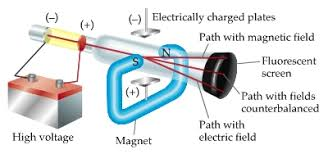
\includegraphics[scale=0.9]{images/08.JJ-Thomson..jpg}
    \caption{Autre schéma réaliste}
    \label{fig:my_label}
\end{figure}

\begin{enumerate}
    
\end{enumerate}
\subsection{Déroulement de l'expérience}
\begin{enumerate}
    \item Le but de l'expérience de J.J. Thomson :
    \begin{enumerate}
        \item trouver le rapport charge - masse des électrons
        \item découvrir l'existence de petites particules chargées négativement, les électrons
    \end{enumerate}
    \item La théorie :
    \begin{enumerate}
        \item formule de l'énergie mécanique (incluant l 'énergie cinétique et celle de l'énergie potentielle)
        \item champs magnétiques et électriques
        \item électricité (loi de Coulomb) 
    \end{enumerate}
    \item Les hypothèses de départ :
    \begin{enumerate}
        \item On suppose que le tube a été mis partiellement mis sous vide.
        \item Il peut y avoir ou non des champs électriques ou magnétiques au niveau des 2 plaques métalliques.
        \item Le voltage du générateur est très élevé.
        \item Les plaques métalliques sont chargées.
    \end{enumerate}
    \item La marche à suivre :
    \begin{enumerate}
    \item On voit, dans le dispositif ci-dessus, un générateur branché à une cathode et à une anode.
    \item Ce générateur va, comme son nom l'indique d'ailleurs, générer/créer des électrons.
    \item S'il n'y avait pas le tube, ses électrons formeront une boucle infinie, en passant sans cesse par la borne positive et par la borne négative. 
    \item Mais vu qu'ils passent par le tube qui a été mis sous vide, ils seront condensé en un faisceau cathodique. 
    \item Ils auront beaucoup d'énergie du fait du haut voltage qu'a le générateur, ils vont donc aller à une vitesse assez élevée.
    \item Les électrons passent ensuite dans le tube et continuent jusqu'aux deux plaques métalliques.
    \item Celle du dessus est chargée négativement et celle du dessous est chargée positivement.
    \item Il y a un aimant en forme de O coupé au milieu pour le tube, qui se situe à l'extérieur du tube donc.
    \item La trajectoire des électrons va monter en présence d'un champ magnétique, va descendre en présence d'un champ électrique et  va aller tout droit quand les champs sont contre-balancés. 
    \item Les plaques métalliques sont chargées.
    \item Sur l'écran fluorescent, il y a des mesures qui relèvent de où a tapé le faisceau cathodique. 
    \end{enumerate}
    \item Les mesures :
    \begin{enumerate}
        \item Comme mesures, J.J. Thomson a mesuré le voltage du générateur.
        \item Il a aussi pris note, grâce ses graduations sur l'écran fluorescent, de là où arrivait le faisceau cathodique.
        \item Et de ces mesures, il a obtenu des résultats que satisfaisants.
    \end{enumerate}
    \item Les résultats :
    \begin{enumerate}
        \item Il a obtenu le rapport de la charge à la masse, chose qui n'a jamais été trouvé avant lui.
        \item Cela lui a permis notamment de trouver l'existence de petites particules chargées négativement qui se trouve dans l'atome. 
    \end{enumerate}
    \item La conclusion :
    \begin{enumerate}
        \item Dans l'atome, il existe des petites particules chargées négativement, en orbite autour du noyau : les électrons.
        \item On a trouvé le rapport charge et masse de l'électron, chose jamais faite avant.
    \end{enumerate}
\end{enumerate}



%\subsection{Le but :}

%Précise les objectifs très généraux à atteindre pendant la séance de TP : quelques lignes suffisent.
%\subsection{La théorie : }
%Doit contenir un développement des bases théoriques sur lesquelles on s'appuie pour réaliser l'expérience. Il s'agit d'un résumé pertinent et personnel.
%\subsection{Les hypothèses de départ : }
%Décrit, point par point quelles sont les conditions dans lesquelles on entend mener l'expérience, dans quelles conditions la loi prédéfinie est valable et par-dessus tout quels sont les phénomènes que l'on négligera.
%\subsection{La marche à suivre : }
%Décrit, comment, au moyen du montage, le but peut être atteint ; elle justifie le montage et la méthode utilisée ; dans cette marche à suivre, on indiquera clairement toutes les grandeurs physiques que l'on va mesurer ainsi que toutes les valeurs provenant de tables numériques.
%\subsection{Les mesures : }
%Sont des valeurs numériques que l'on obtient au moyen d'instruments ; on rassemblera si possible les mesures dans un tableau ; on estimera les incertitudes des mesures.
%\subsection{Les résultats : }
%sont obtenus à partir des mesures, soit par calcul, soit par méthode graphique.\\
%En cas de calcul, on présentera clairement un exemple développé du calcul d'incertitude.\\
%Lorsque l'on tracera un graphique, on indiquera :
%\begin{itemize}
 %   \item un titre
  %  \item les grandeurs reportées sur les axes avec leurs unités
  %  \item des échelles claires et précises sur chaque axe
  %  \item les barres et/ou rectangles d'incertitudes
  %  \item la courbe reliant les valeurs si elle existe
  %  \item la courbe théorique si on la connaît.
%\end{itemize}
%\subsection{La conclusion : }
%Consiste à discuter si le but est atteint ou non ;\\
%on discutera notamment les points suivants :
%\begin{itemize}
%    \item les valeurs obtenues sont-elles en accord avec celles des tables et dans la négative, d'où provient la différence ? En accord signifie compatible avec les incertitudes, d'où  l'importance de ces dernières !
%    \item existe-t-il un modèle physique (une relation mathématique) reliant les grandeurs physiques étudiées ? Laquelle ?
%    \item la méthode choisie est-elle bien adaptée ?
 %   \item le montage permet-il  d'atteindre une bonne précision ?
 %   \item les hypothèses de départ s'avèrent-elles légitimes ?
 %   \item ...
%\end{itemize}

\end{document}